\section{湍流算例}\label{sec:appendix-d-3}

\begin{example}[湍流槽道流]\label{ex:appendix-d-12}
湍流槽道流由如下无量纲不可压缩 Navier--Stokes 方程组描述,其中体力项为 $\bm f=(1,0,0)^\mathsf T$:
\begin{equation}\label{eq:appendix-d-33}
\begin{aligned}
\partial_t\bm u
-2\nabla\cdot\bigl(\mathrm{Re}_{\tau}^{-1}D(\bm u)\bigr)
+(\bm u\cdot\nabla)\bm u+\nabla p
&=\bm f
&&\text{于 }(0,T]\times\Omega,\\
\nabla\cdot\bm u&=0
&&\text{于 }(0,T]\times\Omega,
\end{aligned}
\end{equation}
方程组\hyperref[eq:appendix-d-33]{(D.33)}采用特征长度 $L=1\,\mathrm m$ 和特征速度 $U=1\,\mathrm{m/s}$ 导出.因此,无量纲黏度为 $\nu=\mathrm{Re}_{\tau}^{-1}$(见笔记\hyperref[note:characteristic-scales]{2.19}),流体的运动黏度为 $\mathrm{Re}_{\tau}^{-1}\,\mathrm{m^2/s}$.

文献中对若干 $\mathrm{Re}_\tau$ 给出了基准问题.

\paragraph{$\mathrm{Re}_\tau=180$ 的湍流槽道流.}
计算区域为
\[
\Omega=(-2\pi,2\pi)\times(0,2H)\times
\left(-\frac{2\pi}{3},\frac{2\pi}{3}\right),
\]
其中槽道半宽 $H=1$,$\mathrm{Re}_\tau=180$ 是以半宽、流体运动黏度和剪切速度(或摩擦速度)$U_\tau$ 定义的 Reynolds 数,见笔记\hyperref[note:turbulent-boundary-layers]{8.13}.由
$\mathrm{Re}_\tau=U_\tau H/\nu$,取 $\nu=\mathrm{Re}_\tau^{-1}\,\mathrm{m^2/s}$ 得
$U_\tau=1\,\mathrm{m/s}$,从而无量纲摩擦速度 $u_\tau=U_\tau/U=1$.流向 $x$ 和展向 $z$ 采用周期边界条件;固壁位于 $y=0$ 和 $y=2$,并施加无滑移条件 $\bm u=0$.

初始条件可依据\textcite{Moser1999} 所提供数据文件 \texttt{chan180.means} 中的已知平均速度剖面 $U_{\mathrm{mean}}(y)$ 构造,见图\hyperref[fig:appendix-d-12]{D.12}.对该平均速度剖面作线性插值,并加入随机扰动,例如采用\textcite{Gravemeier2006b} 提出的形式:
\begin{equation}\label{eq:appendix-d-34}
\begin{aligned}
u_1(0;x,y,z)&=U_{\mathrm{mean}}(y)+0.1U_{\mathrm{bulk}}\,\varepsilon(x,y,z),\\
u_2(0;x,y,z)&=0.1U_{\mathrm{bulk}}\,\varepsilon(x,y,z),\\
u_3(0;x,y,z)&=0.1U_{\mathrm{bulk}}\,\varepsilon(x,y,z),
\end{aligned}
\end{equation}
其中
\begin{equation}\label{eq:appendix-d-35}
U_{\mathrm{bulk}}=\frac1H\int_0^H U_{\mathrm{mean}}(y)\,\mathrm dy
\approx15.6803.
\end{equation}
为通过数值积分计算这一数值,$U_{\mathrm{mean}}(y)$ 以三次样条插值.随机函数 $\varepsilon$ 可按 C++ 记法取为
\[
\varepsilon(x,y,z)=\frac{2\,\mathrm{rand}()}{\mathrm{RAND\_MAX}}-1
\in[-1,1].
\]
总之,初始速度场\hyperref[eq:appendix-d-34]{(D.34)}是在插值所得平均速度剖面 $U_{\mathrm{mean}}(y)$ 上加入随机速度扰动,扰动幅度为整体平均速度 $U_{\mathrm{bulk}}$ 的 $20\%$(正、负方向各占 $10\%$).图\hyperref[fig:appendix-d-13]{D.13}给出了计算流场的一个瞬时快照.整体来看,流动方向由左至右.截面上的速度显示,槽道内部的平均流速高于靠近边界处的流速,这符合预期;但边界附近也有涡旋,因此局部流动也会朝反方向运动.
\begin{elegantfigure}[0.55\linewidth]
 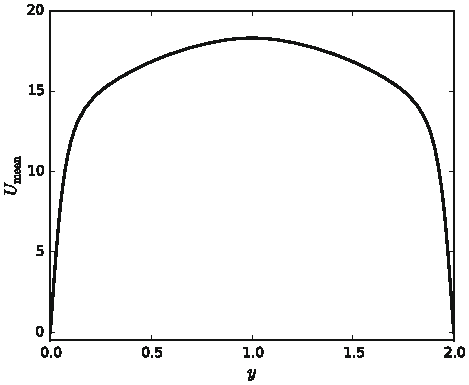
\includegraphics[width=\linewidth]{figures/Appendix_D/Fig_D_12__PDFp773__Bookp768.pdf}
 \captionof{figure}{例题 D.12:据数据文件 \texttt{chan180.means} 绘制的 $\mathrm{Re}_\tau=180$ 湍流槽道流平均速度剖面 $U_{\mathrm{mean}}(y)$.}\label{fig:appendix-d-12}
\end{elegantfigure}
\begin{elegantfigure}[0.94\linewidth]
 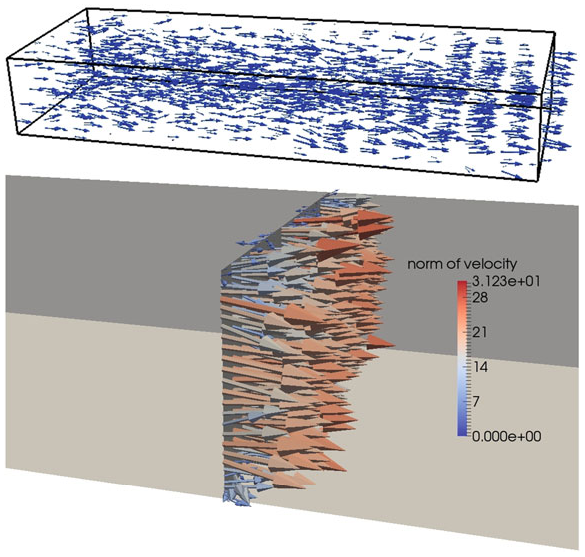
\includegraphics[width=\linewidth]{figures/Appendix_D/Fig_D_13__PDFp774__Bookp769.pdf}
 \captionof{figure}{例题 D.12:$\mathrm{Re}_\tau=180$ 湍流槽道流的速度场快照;上图为整个槽道,下图为垂直于 $x$ 方向的截面(浅灰平面 $y=0$,深灰平面 $z=2\pi/3$).}\label{fig:appendix-d-13}
\end{elegantfigure}

\paragraph{$\mathrm{Re}_\tau=395$ 的湍流槽道流.}
此问题的计算区域为
\[
\Omega=(-\pi,\pi)\times(0,2)\times
\left(-\frac{\pi}{2},\frac{\pi}{2}\right),
\]
固壁仍位于 $y=0$ 和 $y=2$,其余边界仍为周期边界.与 $\mathrm{Re}_\tau=180$ 的情形相同,有 $u_\tau=U_\tau/U=1$.采用\textcite{Moser1999} 的参考平均速度,得到整体平均速度 $U_{\mathrm{bulk}}=17.5452$.初始条件可按 $\mathrm{Re}_\tau=180$ 的方法构造.

\paragraph{感兴趣的统计量.}
用 $\langle\cdot\rangle_t$ 表示时间平均,用 $\langle\cdot\rangle_s$ 表示对空间均匀方向的平均.湍流槽道流的均匀方向是流向 $x$ 和展向 $z$.若时间步等距,有限元速度的时间平均可用算术平均计算:
\[
\langle\bm u^h(t,\bm x)\rangle_t
=\frac1{N_t+1}\sum_{n=0}^{N_t}\bm u^h(t_n,\bm x),
\]
其中 $N_t$ 为时间步数.同理,若均匀方向上的网格等距,空间平均也可用算术平均计算,例如
\[
\langle\bm u^h(t_n,x,y,z)\rangle_s
=\frac1{N_xN_z}\sum_{i=1}^{N_x}\sum_{j=1}^{N_z}
\bm u^h(t_n,x_i,y,z_j),
\]
其中 $N_x$、$N_z$ 分别为 $x$ 和 $z$ 方向的自由度数.

感兴趣的统计量包括平均速度和 Reynolds 应力.前者是一次平均量:
\[
\bm u^h_{\mathrm{mean}}(y)
=\left\langle\left\langle
\bm u^h(t,x,y,z)\right\rangle_s\right\rangle_t,
\]
后者为二次平均量
\begin{equation}\label{eq:appendix-d-36}
T^h_{ij,\mathrm{mean}}
=\left\langle\left\langle u_i^h u_j^h\right\rangle_s\right\rangle_t
-\left\langle\left\langle u_i^h\right\rangle_s\right\rangle_t
 \left\langle\left\langle u_j^h\right\rangle_s\right\rangle_t,
\qquad i,j=1,2,3.
\end{equation}
Reynolds 应力张量的定义见笔记\hyperref[note:les-closure-problem]{8.32}.平均速度中尤为关心第一分量 $u^h_{1,\mathrm{mean}}(y)$.

文献中对 Reynolds 应力的定义并不统一,\textcite{JohnRoland2007} 对此作了讨论.\textcite{Winckelmans2002} 指出,用湍流模拟解计算得到的对角 Reynolds 应力(即式\hyperref[eq:appendix-d-36]{(D.36)}中 $i=j$ 的情形),不能与真实湍流流场的对角应力直接比较.原因在于湍流模型用亚格子尺度应力张量的迹定义修正压力,而模拟中无法获得这一迹(参见亚格子尺度应力偏差部分\hyperref[eq:sgs-deviatoric-part]{(8.61)}).可直接研究的只有所谓 rms(均方根)湍流强度:
\begin{equation}\label{eq:appendix-d-37}
u^h_{i,\mathrm{rms}}
=\left|T^h_{ii,\mathrm{mean}}
-\frac13\sum_{j=1}^{3}T^h_{jj,\mathrm{mean}}\right|^{1/2},
\qquad i=1,2,3.
\end{equation}
\textcite{Winckelmans2002} 还指出,计算二阶统计量\hyperref[eq:appendix-d-36]{(D.36)}和 rms 量\hyperref[eq:appendix-d-37]{(D.37)}时,应计入所用湍流模型的贡献.对于某些模型,这一贡献易于识别和实现,例如式\hyperref[eq:smagorinsky-turbulent-viscosity]{(8.66)}中的 Smagorinsky 模型;另见\textcite{JohnRoland2007}.不过,有些湍流模型的贡献很难纳入.

\paragraph{离散化的若干方面.}
模拟中通常在 $x$、$z$ 方向使用均匀网格,在壁面法向 $y$ 方向使用分级网格,并在靠近壁面处加密;例如可参见\textcite{Gravemeier2006a,Gravemeier2006b} 给出的两种方案.等距时间步长应足够小,以分辨流动的时间变化.\textcite{ChoiMoin1994} 的研究建议满足
\begin{equation}\label{eq:appendix-d-38}
\Delta t^+=u_\tau\mathrm{Re}_\tau\Delta t\le0.4.
\end{equation}

\paragraph{有限元模拟中的一项注意事项.}
由于流动不可压缩,模拟过程中整体平均速度理应保持不变.然而,有限元函数一般并非弱无散,而只是离散无散.因此,有限元离散不会自动保证整体平均速度守恒(这对应质量守恒).\textcite{JohnRoland2007} 提出,可动态调整 Navier--Stokes 方程组的右端项,以校正计算得到的整体平均速度与式\hyperref[eq:appendix-d-35]{(D.35)}之差.流动由压力梯度驱动.设 $U_{\mathrm{bulk,sim}}(t_n)$ 是时刻 $t_n$ 的数值解整体平均速度,则在 $t_{n+1}$ 时刻,方程组\hyperref[eq:appendix-d-33]{(D.33)}的右端项取为
\begin{equation}\label{eq:appendix-d-39}
\bm f
=\begin{pmatrix}1\\0\\0\end{pmatrix}
+\frac{1}{\Delta t_n}
\begin{pmatrix}
U_{\mathrm{bulk}}-U_{\mathrm{bulk,sim}}(t_n)\\0\\0
\end{pmatrix}.
\end{equation}
这里 $\Delta t_n$ 为时间步长.对于具有物理量纲的量,式\hyperref[eq:appendix-d-39]{(D.39)}中的修正项具有正确的物理单位.因此,若 $U_{\mathrm{bulk,sim}}(t_n)<U_{\mathrm{bulk}}$,流动将被加速,数值解的整体平均速度随之增大;若 $U_{\mathrm{bulk,sim}}(t_n)>U_{\mathrm{bulk}}$,驱动力将小于 $1$,数值解的整体平均速度会在下一离散时刻减小.

\textcite{JohnRoland2007} 报告说,若不采用式\hyperref[eq:appendix-d-39]{(D.39)}所示的驱动力动态校正,数值解的整体平均速度可能增大,也可能减小,具体取决于湍流模型.采用这一校正后,整体平均速度仍有一定振荡,但始终接近式\hyperref[eq:appendix-d-35]{(D.35)}给出的值,通常误差小于 $1\%$.
\end{example}

\begin{example}[正方形截面柱绕流,$\mathrm{Re}=22000$]\label{ex:appendix-d-13}
该槽道绕障碍物流动算例由\textcite{Rodi1997}定义.障碍物实际上是立柱,但文献中通常称之为圆柱.图\hyperref[fig:appendix-d-14]{D.14}示意了流动区域的截面,通道高度为 $H=0.4\,\mathrm m$.入口速度为
\begin{equation}\label{eq:appendix-d-40}
\bm u(t,0,y,z)
=\begin{pmatrix}1+0.04\,\mathrm{rand}\\0\\0\end{pmatrix},
\qquad \mathrm{rand}\in[-0.5,0.5].
\end{equation}
入口噪声用于激发湍流.立柱表面施加无滑移条件;在 $x=2.5\,\mathrm m$ 处施加出口条件\hyperref[eq:do-nothing-condition]{(2.37)};其他边界施加自由滑移条件\hyperref[eq:free-slip-condition]{(2.34)}.由于初始条件未知,可先选取某个初始条件,例如将入口条件在初始时刻插值延拓到区域内部,继续模拟至流动充分发展后再计算感兴趣的统计量.该算例描述统计周期流动,图\hyperref[fig:appendix-d-15]{D.15}给出了一个瞬时快照.区域截面示意见图\hyperref[fig:appendix-d-14]{D.14}.
\begin{elegantfigure}[0.7\linewidth]
 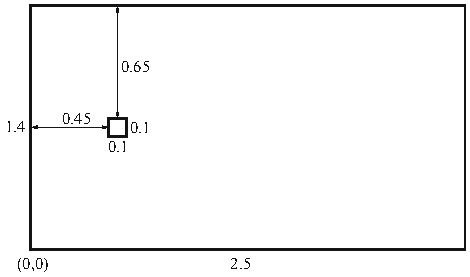
\includegraphics[width=\linewidth]{figures/Appendix_D/Fig_D_14__PDFp777__Bookp772.pdf}
 \captionof{figure}{例题 D.13:流动区域 $x$-$y$ 截面图(长度单位均为米),通道高度 $H=0.4\,\mathrm m$.}\label{fig:appendix-d-14}
\end{elegantfigure}
\begin{elegantfigure}[0.92\linewidth]
 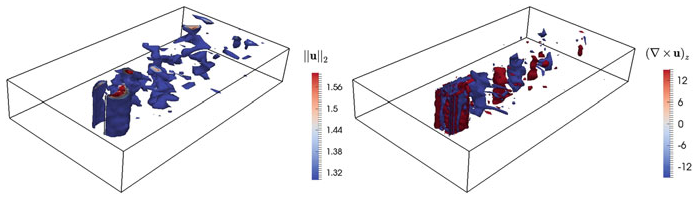
\includegraphics[width=\linewidth]{figures/Appendix_D/Fig_D_15__PDFp778__Bookp773.pdf}
 \captionof{figure}{例题 D.13:速度模等值面(左)和涡量第三分量(见式(3.151),右)的快照;可清楚看到立柱后方的涡脱落.}\label{fig:appendix-d-15}
\end{elegantfigure}

以入口平均速度 $U=1\,\mathrm{m/s}$、立柱边长 $D=0.1\,\mathrm m$ 及运动黏度 $\nu=1/220000\,\mathrm{m^2/s}$ 为尺度,得到 $\mathrm{Re}=UD/\nu=22000$.

与通常的绕体流动一样,感兴趣的量为阻力系数和升力系数.它们可用体积分计算,公式见\hyperref[eq:appendix-d-5]{(D.5)}和\hyperref[eq:appendix-d-8]{(D.8)}.此例取
\[
\begin{aligned}
L=1\,\mathrm m,\qquad V=U,\qquad A=DH,\\
\bm w_{\mathrm{drag}}=\begin{pmatrix}1\\0\\0\end{pmatrix},
\qquad
\bm w_{\mathrm{lift}}=\begin{pmatrix}0\\1\\0\end{pmatrix}.
\end{aligned}
\]
在立柱与自由滑移边界的连接处,$\bm w_{\mathrm{drag}}$ 和 $\bm w_{\mathrm{lift}}$ 应按例题\hyperref[ex:appendix-d-6]{D.6}所述方式设置.Strouhal 数定义为
\[
\mathrm{St}=\frac{DU}{T},
\]
其中 $T$ 为平均周期长度.感兴趣的量包括 Strouhal 数、时间平均阻力系数和升力系数 $\overline{c}_{\mathrm{drag}}$、$\overline{c}_{\mathrm{lift}}$,以及阻力和升力系数的均方根值.对 $n=1,\ldots,N_t$,定义阻力系数和升力系数相对于各自时间平均值的偏差:
\[
\begin{aligned}
\delta_{\mathrm{drag},n}&=c_{\mathrm{drag}}(t_n)-\overline c_{\mathrm{drag}},\\
\delta_{\mathrm{lift},n}&=c_{\mathrm{lift}}(t_n)-\overline c_{\mathrm{lift}}.
\end{aligned}
\]
相应的均方根值为
\[
\begin{aligned}
c_{\mathrm{drag,rms}}&=\left(\frac1{N_t}\sum_{n=1}^{N_t}\delta_{\mathrm{drag},n}^{\,2}\right)^{1/2},\\
c_{\mathrm{lift,rms}}&=\left(\frac1{N_t}\sum_{n=1}^{N_t}\delta_{\mathrm{lift},n}^{\,2}\right)^{1/2}.
\end{aligned}
\]
求和覆盖计算阻力和升力系数的整个时间区间内所有离散时刻.实验参考值见\textcite{Rodi1997}:
\[
\begin{aligned}
\overline c_{\mathrm{drag}}\in[1.9,2.1],\qquad
c_{\mathrm{drag,rms}}\in[0.1,0.2],\\
c_{\mathrm{lift,rms}}\in[0.7,1.4],\qquad
\mathrm{St}=0.132.
\end{aligned}
\]
由于涡脱落具有统计周期性,$\overline c_{\mathrm{lift}}=0$.
\end{example}

\begin{example}[$\mathrm{Re}=40000$ 的壁面立方体绕流]\label{ex:appendix-d-14}
在此算例中,流体不但绕过物体,也会越过物体流动.该问题见\textcite{Hoffman2005,HoffmanJohnson2006};\textcite{Rodi1997} 也提出过类似算例.$z=0$ 处区域底面的示意见图\hyperref[fig:appendix-d-16]{D.16}.立方体高度为 $H$,通道高度为 $2H$.\textcite{Hoffman2005,HoffmanJohnson2006} 的模拟取 $H=0.1\,\mathrm m$.

此算例中没有体力,即 $\bm f=0$.表\hyperref[tab:appendix-d-4]{D.4}给出了平均流向速度的节点值.可将这些值插值到入口边界的自由度上,并加入随机扰动,从而构造模拟入口条件.所得条件与式\hyperref[eq:appendix-d-40]{(D.40)}同型,只需将常数 $1$ 替换为 $u_{1,\mathrm{mean}}$ 的插值值,并可调整随机项前的系数(图\hyperref[fig:appendix-d-17]{D.17}的模拟取 $0.1$).
\begin{elegantfigure}[0.9\linewidth]
 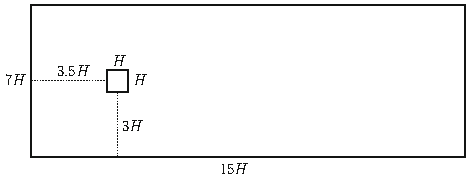
\includegraphics[width=\linewidth]{figures/Appendix_D/Fig_D_16__PDFp779__Bookp774.pdf}
 \captionof{figure}{例题 D.14:$z=0$ 平面上的计算区域底面.}\label{fig:appendix-d-16}
\end{elegantfigure}
\begin{eleganttable}
\captionof{table}{例题 D.14 入口条件的平均速度值.}\label{tab:appendix-d-4}
\begin{tabular}{rrrrrrrr}
\toprule
点 & $u_{1,\mathrm{mean}}$ & 点 & $u_{1,\mathrm{mean}}$ & 点 & $u_{1,\mathrm{mean}}$ & 点 & $u_{1,\mathrm{mean}}$\\
\midrule
0&0&17&1.0315&33&1.0930&49&1.0083\\
1&0.2166&18&1.0461&34&1.0928&50&0.9871\\
2&0.6292&19&1.0587&35&1.0924&51&0.9654\\
3&0.6926&20&1.0661&36&1.0921&52&0.9445\\
4&0.7307&21&1.0723&37&1.0911&53&0.9229\\
5&0.7671&22&1.0770&38&1.0898&54&0.9029\\
6&0.7941&23&1.0813&39&1.0885&55&0.8814\\
7&0.8191&24&1.0843&40&1.0869&56&0.8622\\
8&0.8466&25&1.0868&41&1.0835&57&0.8360\\
9&0.8716&26&1.0890&42&1.0796&58&0.8091\\
10&0.8931&27&1.0890&43&1.0747&59&0.7851\\
11&0.9168&28&1.0890&44&1.0679&60&0.7582\\
12&0.9367&29&1.0890&45&1.0606&61&0.7199\\
13&0.9586&30&1.0900&46&1.0527&62&0.6857\\
14&0.9787&31&1.0930&47&1.0388&63&0.4141\\
15&0.9986&32&1.0930&48&1.0222&64&0\\
16&1.0153&&&&&&\\
\bottomrule
\end{tabular}
\par\smallskip
\parbox{0.95\linewidth}{\centering 入口 65 个等距节点上的平均值,据 J. Hoffman 提供的个人通信.点 0 对应 $z=0$,点 64 对应 $z=2H$.}
\end{eleganttable}

立方体、通道底面和顶面均施加无滑移条件;侧向边界施加自由滑移条件\hyperref[eq:free-slip-condition]{(2.34)};出口可采用 do-nothing 条件\hyperref[eq:do-nothing-condition]{(2.37)}.初始条件未知.可将初始时刻的入口速度插值到区域内部,同时在所有施加无滑移条件的边界上取零,再继续模拟,直至流场充分发展.\textcite{Hoffman2005,HoffmanJohnson2006} 的结果表明,这一状态约在 $3$ 至 $5$ 秒后达到.

入口平均速度约为 $1\,\mathrm{m/s}$.取 Reynolds 数的特征尺度 $U=1\,\mathrm{m/s}$、$H=0.1\,\mathrm m$,并令运动黏度为 $\nu=2.5\times10^{-6}\,\mathrm{m^2/s}$,得到 $\mathrm{Re}=40000$,流动为湍流.再取特征长度 $L=1\,\mathrm m$ 和速度 $U=1\,\mathrm{m/s}$ 推导无量纲 Navier--Stokes 方程\hyperref[eq:time-dependent-ns-strong]{(7.1)},其中无量纲黏度为 $\nu=1/400000$.图\hyperref[fig:appendix-d-17]{D.17}展示了一个流场快照.
\begin{elegantfigure}[0.92\linewidth]
 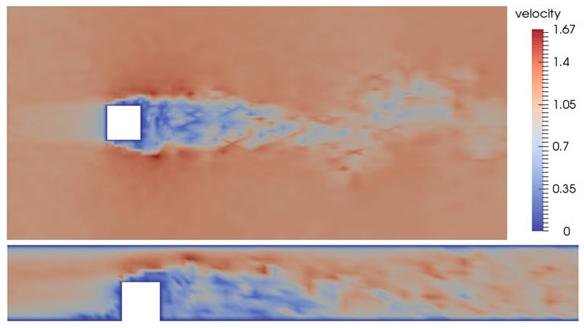
\includegraphics[width=\linewidth]{figures/Appendix_D/Fig_D_17__PDFp780__Bookp775.pdf}
 \captionof{figure}{例题 D.14:$z=H$(上)和 $y=3.5H$(下)截面中的速度模快照.}\label{fig:appendix-d-17}
\end{elegantfigure}

\textcite{Hoffman2005,HoffmanJohnson2006} 的数值研究重点是立方体所受的平均阻力系数.研究使用自适应加密网格和 SUPG 稳定化;具体而言,在式\hyperref[eq:oseen-spg-bilinear-form]{(5.34)}残量中加入 $\partial_t\bm u$,从而形成所谓隐式 LES 模型.网格加密由 DWR 方法控制,见第\hyperref[sec:steady-ns-dwr]{6.4}节.对 $4$ 秒区间作时间平均后,得到平均阻力系数 $\overline c_{\mathrm{drag}}\approx1.5$.流动呈统计周期性,故 $\overline c_{\mathrm{lift}}=0$.计算阻力和升力系数可使用公式\hyperref[eq:appendix-d-5]{(D.5)}和\hyperref[eq:appendix-d-8]{(D.8)}.此例取 $L=1\,\mathrm m$、$V=U$、$A=H^2$,并令 $\bm w_{\mathrm{drag}}=(1,0,0)^\mathsf T$、$\bm w_{\mathrm{lift}}=(0,1,0)^\mathsf T$.
由于物体边界与通道边界相连,实际定义 $\bm w_{\mathrm{drag}}$ 和 $\bm w_{\mathrm{lift}}$ 时,需按笔记\hyperref[note:appendix-d-2]{D.2}作相应修改,例如采用例题\hyperref[ex:appendix-d-6]{D.6}介绍的处理方式.
\end{example}
